\documentclass[12pt, letterpaper]{article}
\usepackage[serbian]{babel}
\usepackage{hyperref}
\usepackage{graphicx}

\begin{document}

\title{AI koji generiše sliku na osnovu teksta}
\author{Budimir Nkola 178/2021\\ \and Trajković Miljan 354/2022 \and Cvejić Miloš 346/2021\\ \and Bajić Bogdan 122/2021}
\maketitle

\begin{abstract}
    Ovaj rad je napisan sa ciljem da vas upozna sa jednom aktuelnom primenom veštačke inteligencije. Ukratko će vam biti objašnjeno kako se ovakav sistem razvija, kako funkcioniše i kako ga i vi možete koristiti, a zatim vas će i sprovesti kroz probleme koje donosi sa sobom.
\end{abstract}
\begin{tableofcontents}
\end{tableofcontents}

\pagebreak 

\section{Uvod} 

\subsection*{Veštačka inteligencija} 

Veštačka inteligencija predstavlja podoblast računarstva koja omogućava računarima da realizuju funkcije koje su karakteristika ljudskog razmišljanja, odnosno da što vernije imitiraju rad ljudskog mozga. Počela je da se razvija tokom druge polovine dvadesetog veka. Neka od čestih mesta na kojima se upotrebljava veštačka inteligencija su obrada podataka, prepoznavanje slika, video igre, medicina, napredni internet pretraživači, sistemi preporuke, proizvodnja bespilotnih letelica i autonomnih automobila, generisanje slika, kao i još mnogo drugih.  

  

Mašinsko učenje predstavlja podoblast veštačke inteligencije. Ono omogućava da računar “nauči” zadati šablon koji dobija kroz milione podataka i upotrebi ga kako bi mogao da oponaša taj isti tip ponašanja.   

  

Pristupi mašinskom učenju se generalno dele u tri različite kategorije, u zavisnosti od prirode signala ili povratne informacije dostupne sistemu učenja. To su: učenje pod nadzorom (eng. supervised learning), polunadgledano učenje (eng. semi-supervised learning), učenje bez nadzora (unsupervised learning) i učenje potkrepljenjem (reinforcement learning).  

  

Učenje pod nadzorom je paradigma mašinskog učenja kod koje postoji nadgledač koji predstavlja učitelja. Kod ovog tipa učenja, obučavamo računar koristeći podatke koji su ispravno označeni, nakon čega mu dajemo pristup novim podacima, koje on treba da analizira, prepozna i da zna šta treba da radi sa njima. Učenje bez nadzora je paradigma mašinskog učenja kod koje se računar obučava koristeći informacije koje nisu označene. Zadatak računara je da grupiše zadate podatke prema njihovim sličnostima, bez ikakve prethodne obuke. Učenje potkrepljenjem predstavlja paradigmu mašinskog učenja koja podseća na treniranje kućnog ljubimca. Radi se o nagrađivanju računara kada je radnja koju je učinio adekvatna. Na prvi pogled to podseća na učenje pod nadzorom, ali za razliku od tog tipa, kod učenja potkrepljenjem računar nema podatke koje koristi za buku, već uči iz sopstvenog iskustva \cite{kljucDva}. 

  

\subsection*{Šta je AI generator slika} 

AI generator slika predstavlja program koji generiše sliku na osnovu zahteva zadatog u obliku teksta koristeći veštačku inteligenciju. To funkcioniše tako što generator slika ima pristup bazi podataka u kojoj se nalazi veliki broj različitih slika, na osnovu kojih on uči da generiše nove slike. Kada generator slika dobije opis slike koju treba da generiše, on u bazi podataka proverava slike sa sličnim opisom i na osnovu njih generiše sliku koja podseća na njih.    

Neki od poznatih programa za generisanje slika na osnovu zadatog teksta su: 

\begin{itemize} 
\item[-] Dall-E  
\item[-] Jasper Art
\item[-] Starry AI 
\item[-] Midjourney
 
\end{itemize} 

\section{Kako funkcionišu AI generatori slika}
\subsection*{Preteče današnjih generatora}
Mnogi modeli veštačke inteligencije pa tako i generatori slika na osnovu teksta poput \textbf{DALL-E 2} i drugih, zasnovani su na prethodnim istraživanjima i prethodnim modelima.
Generisanje slika razvijalo se linearno i to prvobitno koriscenjem mreža koje koriste metode suparničkog učenja odnosno “Generative adversarial network” (GANs).

GANs su modeli mašinskog učenja obično sačinjeni od dve mreže, \textit{diskriminatora} i \textit{generatora}, koje međusobnim intereagovanjem treniraju jedna drugu. Naime, ako uzmemo na primer generisanje slika, zadatak diskriminatora je da što sigurnije i preciznije odredi da li je njemu zadata slika, prava fotografija iz neke baze podataka ili je to generisana slika. Sa druge strane, zadatak generatora je da prevari diskriminatora, odnosno da što bolje nauči šta sliku čini “pravom” i tako napravi sliku za koju se ne može utvrditi da li je ona prava ili ne. U tom slučaju interakcija ove dve mreže i njihovo treniranje se može posmatrati kao minimaks igra u kojoj se diskriminator trenira da maksimalno uveća verovatnoću tačnog određivanja klase slika, dok se generator trenira da maksimalno umanji verovatnoću da slike koje je generisao budu klasifikovane od strane diskriminatora kao generisane slike \cite{gan}.

Ključna razlika između ovako opisanih mreža i najnovijih AI generatora slika je ta što se klasični GAN modeli obično razvijaju za neku konkretnu kategoriju fotografija(npr. popularni generator ljudskih lica) dok na drugoj strani generatori poput DALL-E 2 su mnogo opštije namene.

Arhitekture najnovijih generatora zasnovane su na jednoj od novijih tehnika nazvanoj difuzija(eng. diffusion) koja je inspirisana oblašću iz fizike - neravnotežna termodinamika. Naime, ako sipamo kap farbe u vodu, zakoni fizike nalažu da će ta kap da \textit{difunduje}\footnote{Difundovanje - proces spontanog raspršivanja materije i energije, prelazak iz zone više u zonu niže energije ili koncentracije} sve dok ne dođe u ravnotežu. Ovaj proces u prirodi je ireverzibilan. U mašinskom učenju, modeli difuzije nastoje da reše upravo ovaj problem, odnosno da nađu način kojim mogu doći do početne kapi farbe \cite{difvideo}.

\subsection{Pregled arhitekture DALL-E 2 softvera}

Za pocetak posmatraćemo takozvanu CLIP mrežu (skraćeno od Contrastive Language–Image Pre-training). Njen osnovni zadatak je da zadatu sliku poveže sa odgovarajućim unetim opisom. Primetimo da se na neki način generisanje slika može smatrati suprotnim procesom od pomenutog. Na ulazu CLIP mreže nalaze se dva kodera koji kodiraju zadatu sliku i njen opis u odgovarajući \textit{imbeding}\footnote{imbeding (eng. embedding) - rezultat preslikavanja skupa informacija u računarski zapis, vektor}, zasebice. Prilikom treniranja, CLIP nastoji da pomenute kodere nauči da imbeding slike i imbeding njenog opisa budu što sličniji jedan drugom\cite{openai_dali}.


Sama arhitektura Dall-E 2 softvera se sastoji iz dva dela: Prvi deo čini mreža prior\footnote{prior - označava ono što je pre nečega po redu ili hronološki.} koji na ulazu prima tekst imbeding (formiran CLIP kodiranjem tekstualnog opisa željene slike) koji preslikava u imbeding slike koji prosleđuje drugom delu ovog generatora - dekoderu. Sada dolazimo do ključnog značaja CLIP mreže. OpenAI tim se zapitao, da li je prior u ovom pristupu uopšte potreban. Iz tog razloga pokušali su da dekoderu proslede samo tekstualni opis, zatim tekstualni opis i tekst imbeding, a na kraju i imbeding slike dobijen pomoću prior-a. Iz tog eksperimenta su zaključili da slike generisane imbedingom slike daju značajno bolje rezulate u odnosu na druga dva slučaja.

Dekoder je generativni model realizovan pomenutom tehnikom difuzuje. Naime, slike se generišu iz nasumične količine \textit{Gausovog šuma}\footnote{Gausov šum (engl. Gaussian noise) - šum raspoređen korišćenjem Gausove normalne raspodele}. Zadatak generatornog dela je da pretpostavi koliko šuma je na slici i otkloni ga. Ovo je vrlo težak problem koji se uspešno rešava upravo difuzno i to na sledeći način: Otklanjanje šuma vrši se iterativno. U svakoj iteraciji pretpostavlja se koliko šuma je na slici koji se otklanja, a zatim se na dobijenu sliku dodaje skoro malo manja količina Gausovog šuma od prethodnog i prelazi u sledeću iteraciju. Kako bi dekoder znao šta uopšte treba da generiše, odnosno “šta se nalazi ispod šuma” prosleđuje mu se uslov. Kod ranijih projekata kao što su GLIDE i DALL-E \cite{openai_glide}, dekoderu se kao uslov direktno prosleđivao tekstualni opis željene slike. Dok se kod ovog modela zahvaljujući CLIP i prior mreži generatoru dodatno prosleđuju CLIP imbeding slike i teksta. Generisanje različitih slika i variranje u odnosu na jednu generisanu sliku se postiže tako što se dobijena slika propušta kroz CLIP koder kako bi se dobio njen imbeding slike, a onda se proces generisanja ponavlja sa novonastalim imbedingom. Na ovaj način dobija se slika koja ima iste elemente i stil prethodne slike, a različit raspored i neke trivijalne detalje koji se gube CLIP kodiranjem. Izlaz opisanog dela dekodera je slika formata 64x64\cite{openai_dali}.

Zato se na samom kraju ovog generatora slika rezolucije 64x64 prolazi kroz jos dva ekspanzivna koraka kojim se slika dovodi na rezoluciju 1024x1024. Ovi koraci su takođe realizovani difuznim tehnikama što doprinosi tome da slika na izlazu ima više detalja i bude maksimalno fotorealistična.

\begin{figure}[htp]
\centering
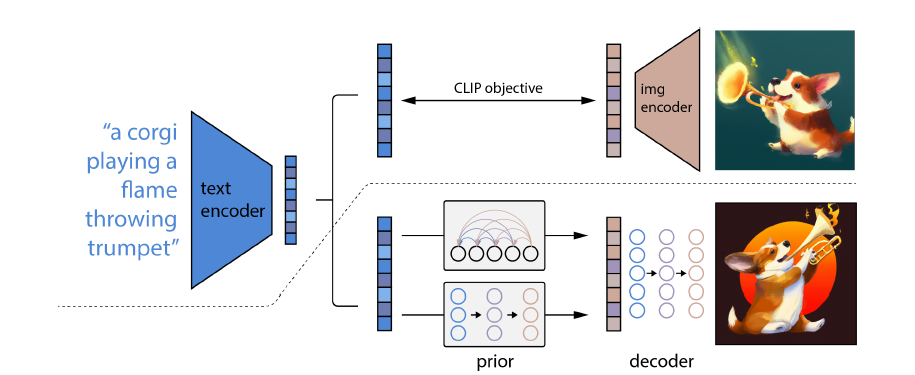
\includegraphics[width=1\textwidth]{dalle2.png}
\caption{Prikaz DALL-E 2 modela iz ptičije perspektive}
\label{fig: dalle2slika}
\end{figure}

\section{Treniranje AI generatora slika}

Za trening softvera kao što je generator slika neophodne su ogromne baze podataka slika koje su pažljivo birane za ovaj trening. Naravno, kreiranje ovakvih baza podataka i prikupljanje slika generalno zahteva veliki broj ljudi. Jedna od najzahtevnijih baza jeste The ImageNet baza slika na kojoj je radilo preko 25 hiljada ljudi koji su skupili 14 miliona slika na kojima se može naći dvadeset dve hiljade različitih objekata\cite{clip}. 

Već smo pričali o CLIP mreži. Tokom njenog treniranja ona prima parove slika i njihovih opisa. Te parove mreža pronalazi na internetu. Možemo primetiti da slike dobijene Gugl pretragom, kao i slike na društvenim mrežama poput Instagrama i Tvitera gotovo uvek imaju opise i lako im se pristupa. Samim tim trošak na građenje iscrpnih baza slika potpuno je prevaziđen.

Treniranje dekodera svodi se na treniranje difuznog modela. Bitno je pomenuti jednu difuznu tehniku zvanu navođenje bez klasifikatora(eng. Classifier-free guidance). Ova tehnika podrazumeva da se generatoru u određenom broju slučaja prosleđeni CLIP imbeding postavljaju na nulu, čime je generator forsiran da napravi sliku samo na osnovu teksta. A tokom treniranja 50\% posto generacija izvršava se bez teksta, odnosno samo pomoću CLIP imbedinga\cite{openai_dali}.

Takođe, tokom treniranja mreža koje sliku rezolucije 64x64 proširuju na sliku rezolucije 1024x1024, slike koje dolaze na ulaz mogu biti malo zamućene korišćenjem Gausove normalne raspodele. Kao što smo rekli baš zbog ovih difuznih tehnika na izlazu dekodera dobijamo sliku rezolucije 1024x1024 koja sadrži puno detalja.

\section{Kako bilo ko može da koristi AI za generisanje slika}
Veštačka inteligencija koja generiše slike bila je jedna od gorućih tema u vestima ove godine zbog izuzetno brzog napretka ali i etičkih problema koje može da donese. Međutim, zašto bi, i kako, mogli da koristimo ove novotarije?

Motivacija za korišćenje je sposobnost AI-a da generiše realistične, ili čak, hiperrealistične slike koje se može koristiti u svrhu razvoja moderne umetnosti, i konstantnog napredovanja AI-a koje mu dozvoljava da stalno proizvodi nove ideje, koje mogu biti ogromna inspiracija.


Dok su neki od izazova da bez obzira na kvalitet slika, one ipak iza sebe neće imati priču ili emocije, to što AI stvara isključivo na osnovu podataka koje poseduje što može dovesti do manjka originalnosti. I najvažnije, etički problemi  i razni načini zloupotrebe veštački generisanih slika. 

\subsection{DALL-E 2}
\textbf{DALL-E 2} kompanije OpenAI jedno je od glavnih imena u ovom prostoru. Čitav proces generisanja je zapravo prilično jednostavan – unesemo opis željene stvari i dobijemo sliku toga.

Da biste koristili DALL-E 2, sve što je potrebno jeste da se ulogujete na sajt. Dužina samog opisa tj. \textit{prompt-a}\footnote{eng. to prompt - navesti} je 400 karaktera, a sam prompt može da primi \textit{sadržaj} i \textit{modifikatore}. Sadržaj je npr. \textit{"usamljeni astrounaut na Marsu"}, a modifikator \textit{"misteriozno, sa puno boja, hiperrealistično"} (naravno, podrazumeva se da se reči unose na engleskom). 

\subsection{Midjourney}
\textbf{Midjourney} je AI alatka koja funkcioniše isključivo na digitalnoj platformi Discord\footnote{Discord(transkribovano Diskord) je platforma namenjena za komunikaciju.}. Ako imate nalog na Diskordu, sve što treba da uradite jeste da se prijavite preko zvaničnog sajta za Midjourney. Sam  AI funkcioniše slično kao i prethodno pomenuti DALL-E 2 samo što se ceo proces ne odvija na sajtu već u aplikaciji. Midjourney uvek generiše 4 slične slike. Ako vam se rezultat dopao, možete da povećate rezoluciju slike, ili da tražite da generiše novu. Ono po čemu se razlikuje od DALL-E 2 je što se manje fokusira na realizam a više na maštovitiju i raznobojniju kreaciju.

\begin{center}
\begin{tabular}{ |c|c|c| } 
 \hline
 DALL-E 2 & \href{https://openai.com/dall-e-2/}{openai.com/dall-e-2} \\
 Midjourney & \href{https://www.midjourney.com/}{midjourney.com} \\
 \hline
\end{tabular}
\end{center}

\section{Etički problemi sa veštačko inteligentnim generatorima slika}

AI generatori slika mogu doprineti diskriminaciji tako što oponašaju štetne stereotipe koje je AI prikupio u kolekcijama podataka, koji sami imaju predrasude iz svakodnevnog života.

U svom članku Rune Klingenberg Hansen nudi sledeća rešenja \cite{kljuc1}. Problem se može korigovati zabranjivanjem određenih reči ili nasumičnim dodavanjem prefiksa kao što su: žena/muškarac/trans, crna/žuta/braon osoba, itd.). Ali nekada automatsko dodavanje dodatnih reči može negativno uticati umesto da reši problem. Npr. dodavanje reči žena za neke termine koji se koriste za osobe svih polova ili dodavanje reči crnac kada se spominju bande/kartele.

Još jedan problem je mogućnost veštačke inteligencije da generiše lažne informacije. To je upravo razlog zašto DALL-E \cite{poznate} ne dozvoljava generisanje slika sa poznatim osobama.

Ali najstrašnije stvar jeste da ova tehnologija može u potpunosti uništiti naše poverenje u slike kao verodostojan dokaz. Zbog straha da su slike lažne, jer generator slika nam omogućava da kreiramo fotorealistične slike. Opasnost od ovog scenarija se može umanjiti korišćenjem tehnologija koje imaju sposobnost detektovanja lažnih slika.



\subsection{Problem autorskih prava}

Generatori slika svima nama dozvoljavaju da kreiramo potpuno nove slike i da ih koristimo u komercijalne i lične svrhe, ali onda se javlja pitanje ko polaže autorska prava nad tim generisanim slikama. Da li osoba koja je okucala tekst i pritisnula dugme za generisanje, da nije algoritam koji je izgenerisao sliku ili pak kompanija koja je kreirala algoritam?

Pitanje autorskih prava je široka tema. Svakodnevno postoje rasprave o tome ko polaže autorka prava. Trenutno ne postoji prihvaćeni odgovor na ovo pitanje, i dalje rasprava je potrebna. 

Generatori slika stvarno kreiraju problem celokupnoj kreativnoj industriji, ali treba na veštačku inteligenciju posmatrati kao na još jednu alatku koju umetnik može da koristi.

\section{Zaključak}

Dakle, znamo šta je veštačka inteligencija, kako se ona može upotrebiti(ali i zloupotrebiti) za generisanje slika, kako radi, kao i par naših omiljenih primera. Naravno, i dalje postoje mnoga ograničenja, ali i mogućnosti za napredak u oblasti AI-a. 

Oduprećemo se želji da vodimo debatu o tome kako će sve ovo uticati na kreativnu industriju. Međutim, istorija nam sugeriše da pojava novih alata ima tendenciju da proširi definiciju umetnosti, odnosno \textit{"umetnost nije mrtva, samo je mašinski generisana"} \cite{clanaknov}.

\begin{thebibliography}{10}

\bibitem{kljucDva} Dostupno na adresi https://www.cse.unsw.edu.au/~cs9417ml/RL1/introduction.html 

\bibitem{gan} Stanislav Frolov, Tobias Hinz, Federico Raue, Jörn Hees, Andreas Dengel, Adversarial text-to-image synthesis: A review. Dostupno na adresi https://www.sciencedirect.com/science/article/pii/S0893608021002823

\bibitem{openai_glide} Alex Nichol, Prafulla Dhariwal, Aditya Ramesh, Pranav Shyam, Pamela Mishkin, Bob McGrew, Ilya Sutskever, Mark Chen, GLIDE: Towards Photorealistic Image Generation and Editing with Text-Guided Diffusion Models. Dostupno na adresi https://arxiv.org/abs/2112.10741/

\bibitem{openai_dali} Aditya Ramesh, Prafulla Dhariwal, Alex Nichol, Casey Chu, Mark Chen, Hierarchical Text-Conditional
Image Generation with CLIP Latents. Dostupno na adresi https://cdn.openai.com/papers/dall-e-2.pdf/

\bibitem{difvideo} AssemblyAI, Diffusion models explained in 4-difficulty levels. Dostupno na adresi https://www.youtube.com/watch?v=yTAMrHVG1ew\&t=53s/

\bibitem{clip} OpenAI, CLIP: Connecting
Text and Images. Dostoupno na adresi https://openai.com/blog/clip/

\bibitem{kljuc1} Rune Klingenberg Hansen, AI Image Generator: This Is Someone Thinking About Data Ethics. Dostupno na adresi https://dataethics.eu/ai-image-generator-this-is-someone-thinking-about-data-ethics/

\bibitem{poznate} DALL-E 2 Content policy. Dostupno na adresi https://labs.openai.com/policies/content-policy

\bibitem{clanaknov} Guido Appenzeller, Matt Bornstein, Martin Casado, Yoko Li, \textit{Art isn't dead, it's just machine-generated}

\end{thebibliography}

\end{document}
